% =============================================================
% 4.2 การออกแบบเนื้อเรื่องของเกม (Storyboard)
% โครงงาน: การออกแบบและพัฒนาเกมเดินเรือด้วยระบบสั่งการด้วยเสียงเพื่อส่งเสริมทักษะการสื่อสาร
% =============================================================

\section{การออกแบบเนื้อเรื่องของเกม (Storyboard)}

ผู้เล่นจะได้สวมบทบาทเป็น \textbf{``กัปตันเรือ''} (Captain) ผู้รับผิดชอบในการนำเรือบรรทุกสินค้าเดินทางฝ่าน่านน้ำที่เต็มไปด้วยอุปสรรคและความท้าทาย โดยเนื้อเรื่องจะสะท้อนถึงการฝึกฝนทักษะการสื่อสารภาษาอังกฤษและการตัดสินใจภายใต้สถานการณ์กดดัน ผ่านการสั่งการลูกเรือปัญญาประดิษฐ์ (AI Crew) 2 คน ได้แก่ ต้นกลเรือ (Chief Engineer) ชื่อ Harris และพลถือท้ายและยามระวังหน้า (Helmsman and Lookout) ชื่อ Finn เกมมี 2 โหมด ได้แก่ โหมดเนื้อเรื่อง (Story) ซึ่งมี 3 บท บทละ 3 ภารกิจ โดยแต่ละภารกิจใช้แผนที่คงที่ และโหมดเดินเรืออิสระ (Free Sail) ซึ่งผู้เล่นเลือกงานขนส่งที่อู่ต่อเรือและเดินเรือในด่านที่สุ่มสร้างใหม่ทุกครั้ง ลำดับเหตุการณ์และเนื้อเรื่องภายในเกมแสดงดังตารางที่ \ref{tab:storyboard}--\ref{tab:storyboard2}

\begin{table}[!htbp]
\centering
\caption{ลำดับเหตุการณ์และสตอรี่บอร์ดของเกมเดินเรือ (ฉากที่ 1--3)}
\label{tab:storyboard}
\begin{tabular}{|L{3.98cm}|L{9.74cm}|}
\hline
\textbf{ภาพประกอบ} & \textbf{คำอธิบายเนื้อเรื่องและเหตุการณ์} \\
\hline
\vspace{0.1cm}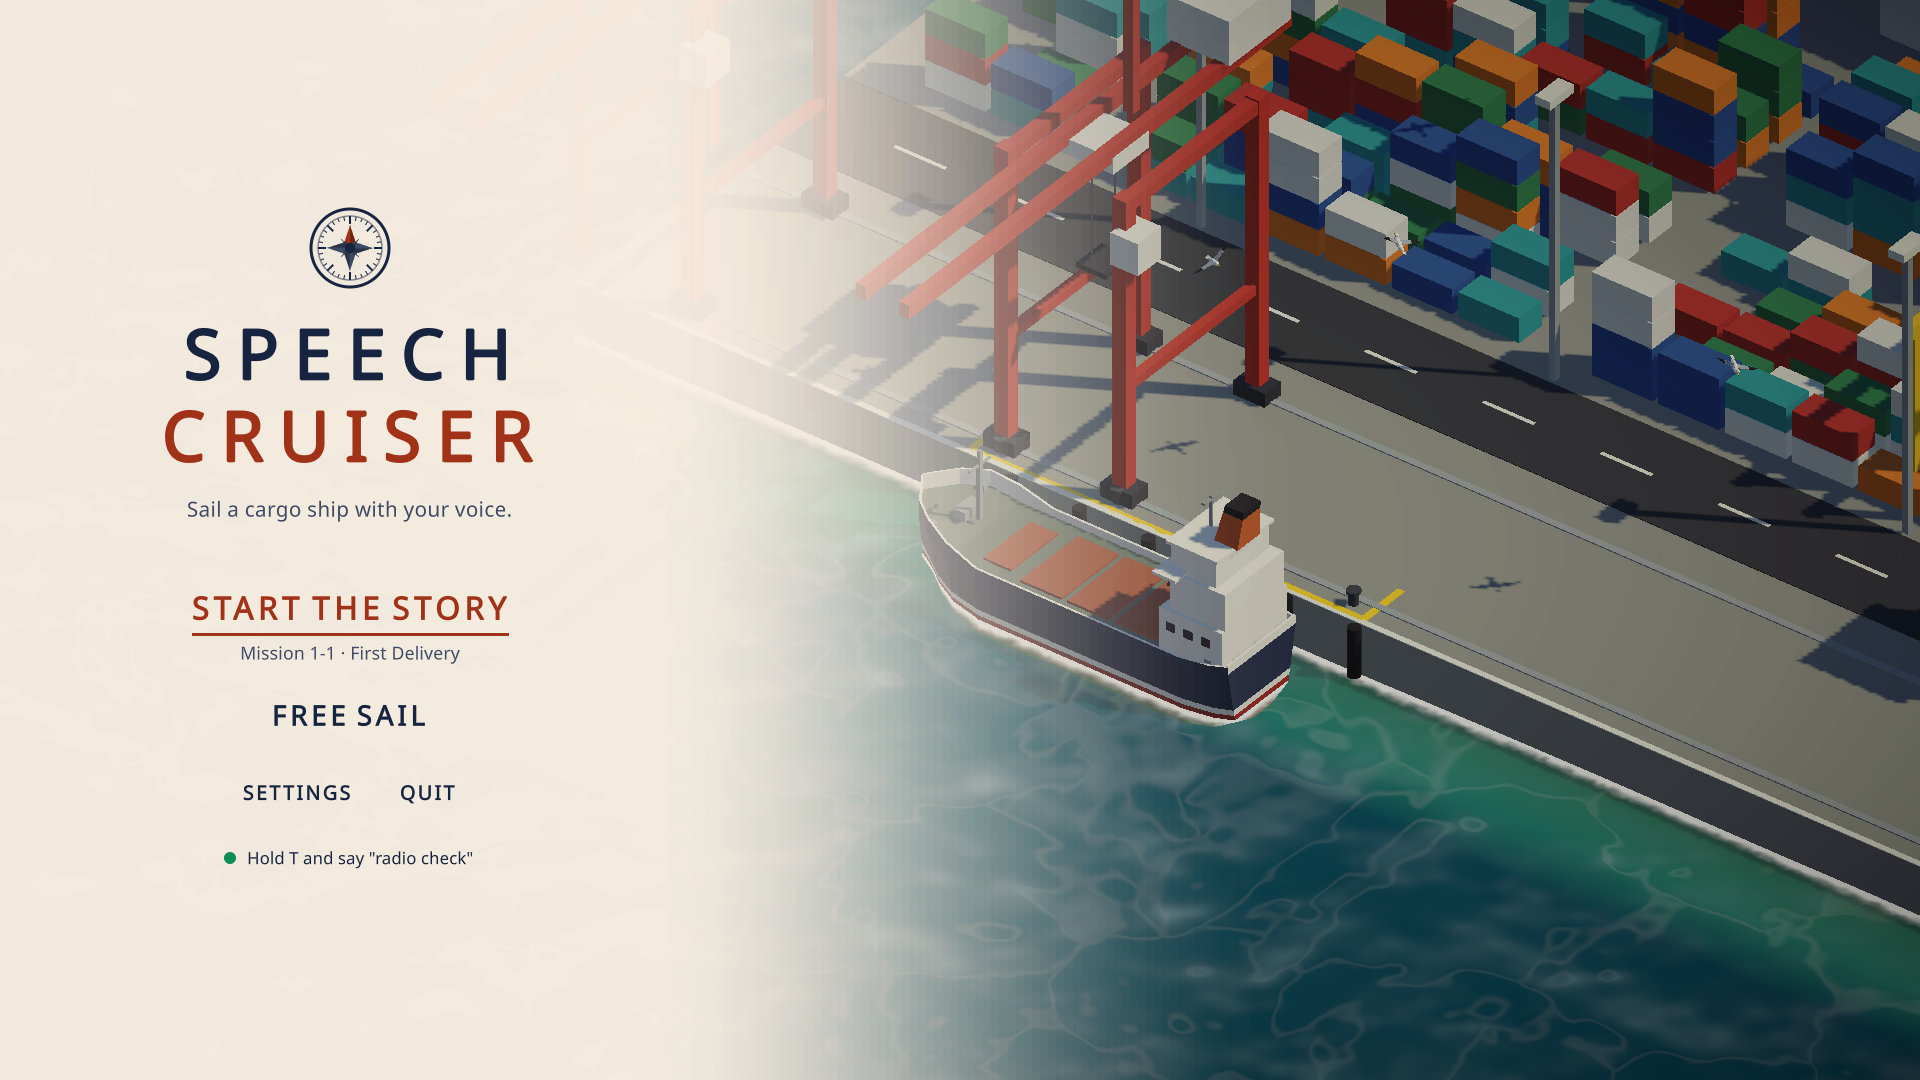
\includegraphics[width=\linewidth]{Document/GameDev/images/MainMenu.png}\vspace{0.1cm} &
\textbf{ฉากที่ 1: เมนูหลัก}\newline
เกมเริ่มที่เมนูหลัก ผู้เล่นเลือกโหมดเนื้อเรื่องหรือเดินเรืออิสระ ปุ่มโหมดเนื้อเรื่องแสดงชื่อภารกิจถัดไป และด้านล่างแสดงสถานะไมโครโฟนพร้อมชวนให้ผู้เล่นทดสอบวิทยุก่อนเริ่มเล่น \\ \hline

\vspace{0.1cm}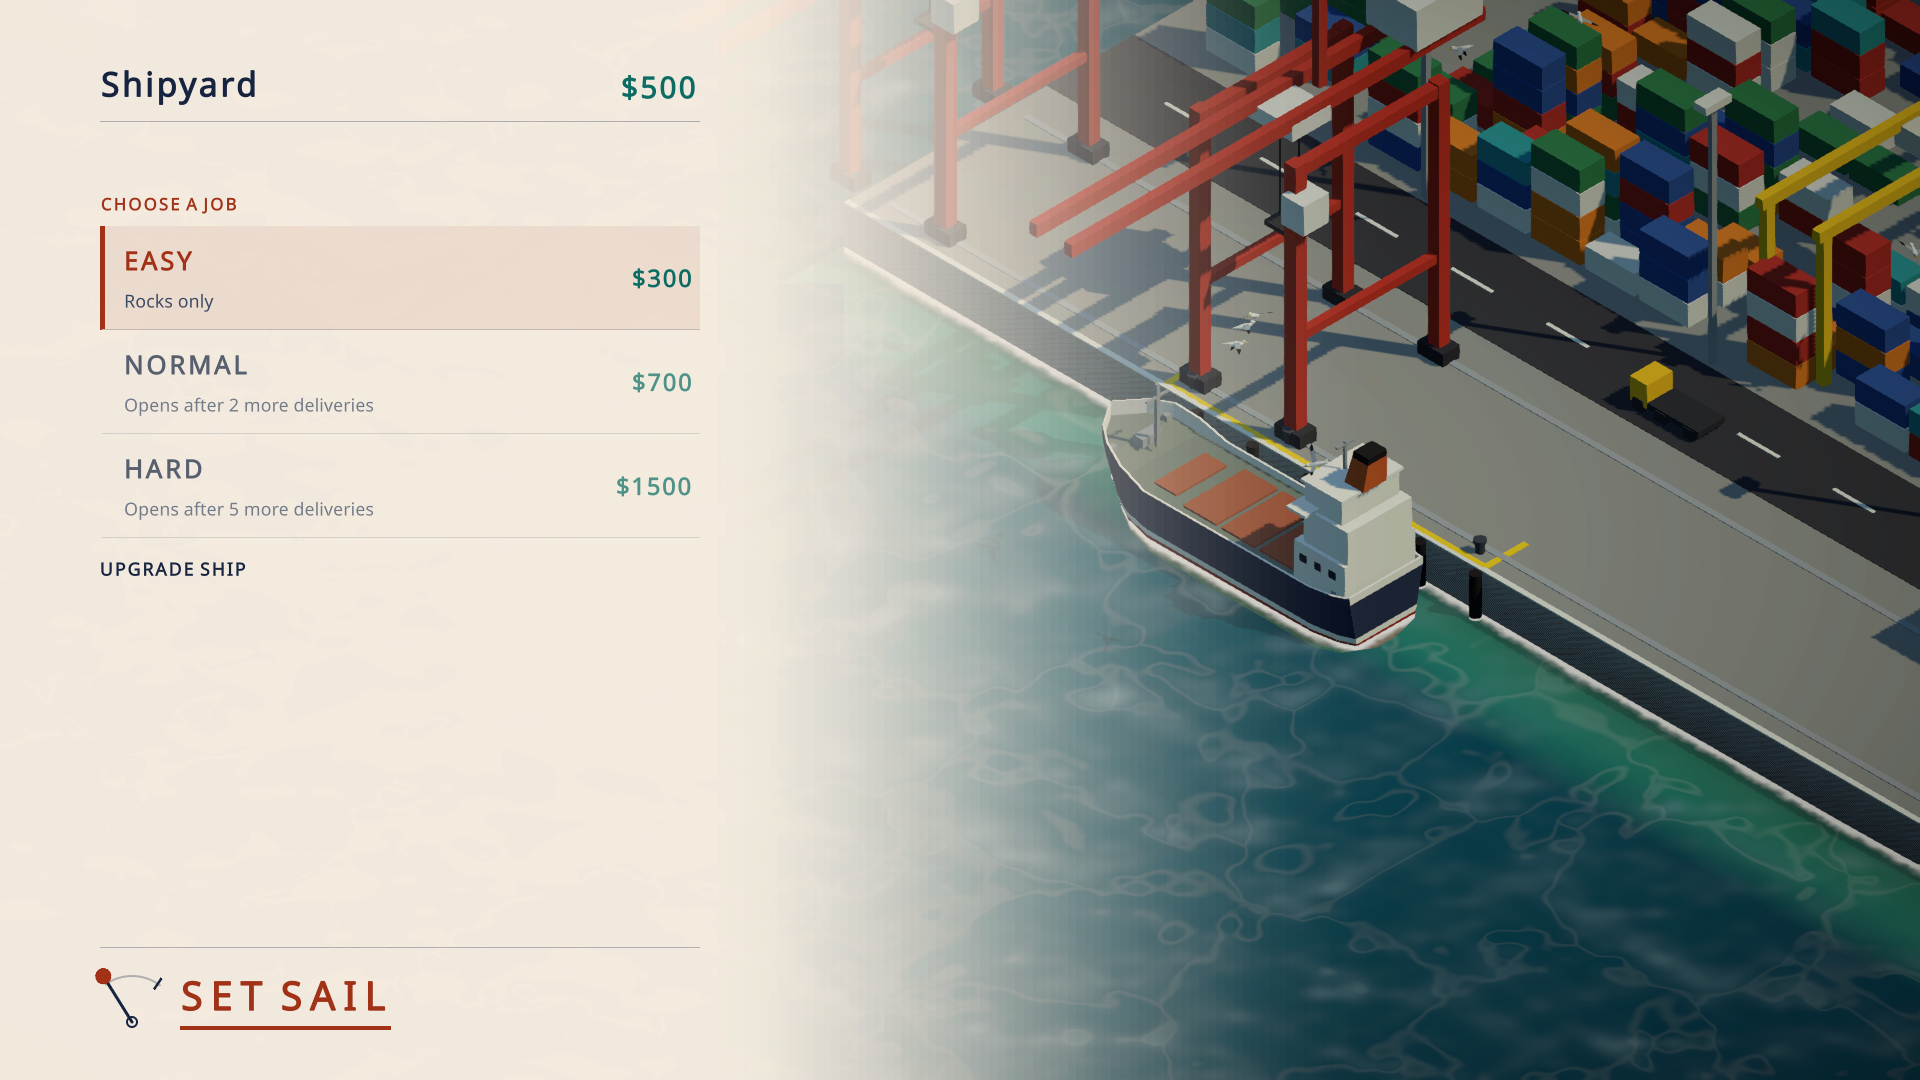
\includegraphics[width=\linewidth]{Document/GameDev/images/Shipyard.png}\vspace{0.1cm} &
\textbf{ฉากที่ 2: การรับมอบหมายภารกิจ}\newline
ในโหมดเดินเรืออิสระ ผู้เล่นเริ่มต้นในฐานะกัปตันเรือที่อู่ต่อเรือ (Shipyard) พร้อมเสียงคลื่นและนกนางนวลเพื่อสร้างความรู้สึกดื่มด่ำ (Immersion) กัปตันเลือกงานขนส่งสินค้าตามระดับความยาก แล้วสั่งออกเรือ (Set Sail) เพื่อนำเรือไปเทียบท่าปลายทางอย่างปลอดภัย ส่วนในโหมดเนื้อเรื่อง ภารกิจเริ่มจากบทสนทนาแนะนำเรื่องราวก่อนออกเรือ \\ \hline

\vspace{0.1cm}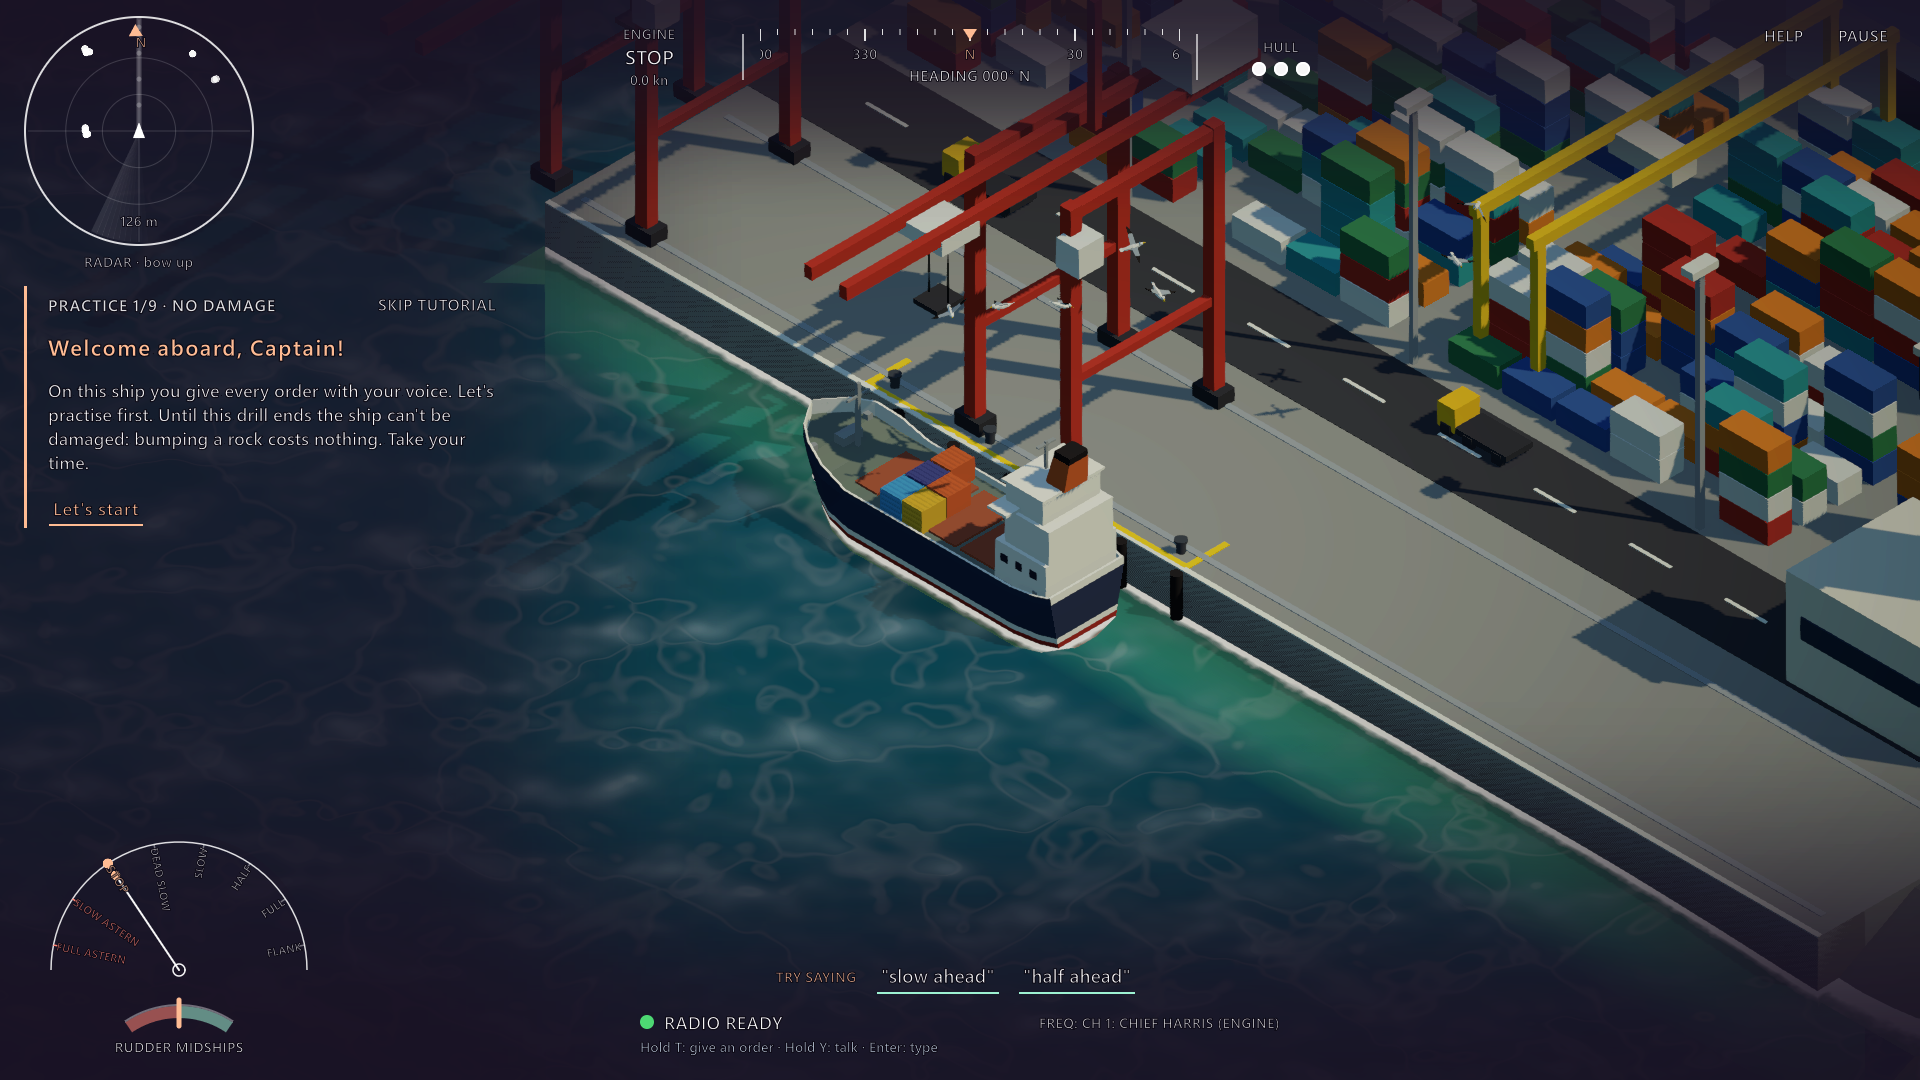
\includegraphics[width=\linewidth]{Document/GameDev/images/Tutorial.png}\vspace{0.1cm} &
\textbf{ฉากที่ 3: การแนะนำลูกเรือปัญญาประดิษฐ์}\newline
แนะนำลูกเรือทั้งสองตำแหน่ง ได้แก่ ต้นกลเรือผู้รอรับคำสั่งเครื่องยนต์และความเร็ว และพลถือท้ายผู้รอรับคำสั่งหางเสือและคอยแจ้งเตือนภัยจากเรดาร์ ในการเดินเรือครั้งแรก เกมเริ่มบทฝึกสอน (Tutorial) การออกคำสั่งเสียงภาษาอังกฤษพื้นฐาน \\ \hline
\end{tabular}
\end{table}

\begin{table}[!htbp]
\centering
\caption{ลำดับเหตุการณ์และสตอรี่บอร์ดของเกมเดินเรือ (ฉากที่ 4--6)}
\label{tab:storyboard2}
\begin{tabular}{|L{3.98cm}|L{9.74cm}|}
\hline
\textbf{ภาพประกอบ} & \textbf{คำอธิบายเนื้อเรื่องและเหตุการณ์} \\
\hline
\vspace{0.1cm}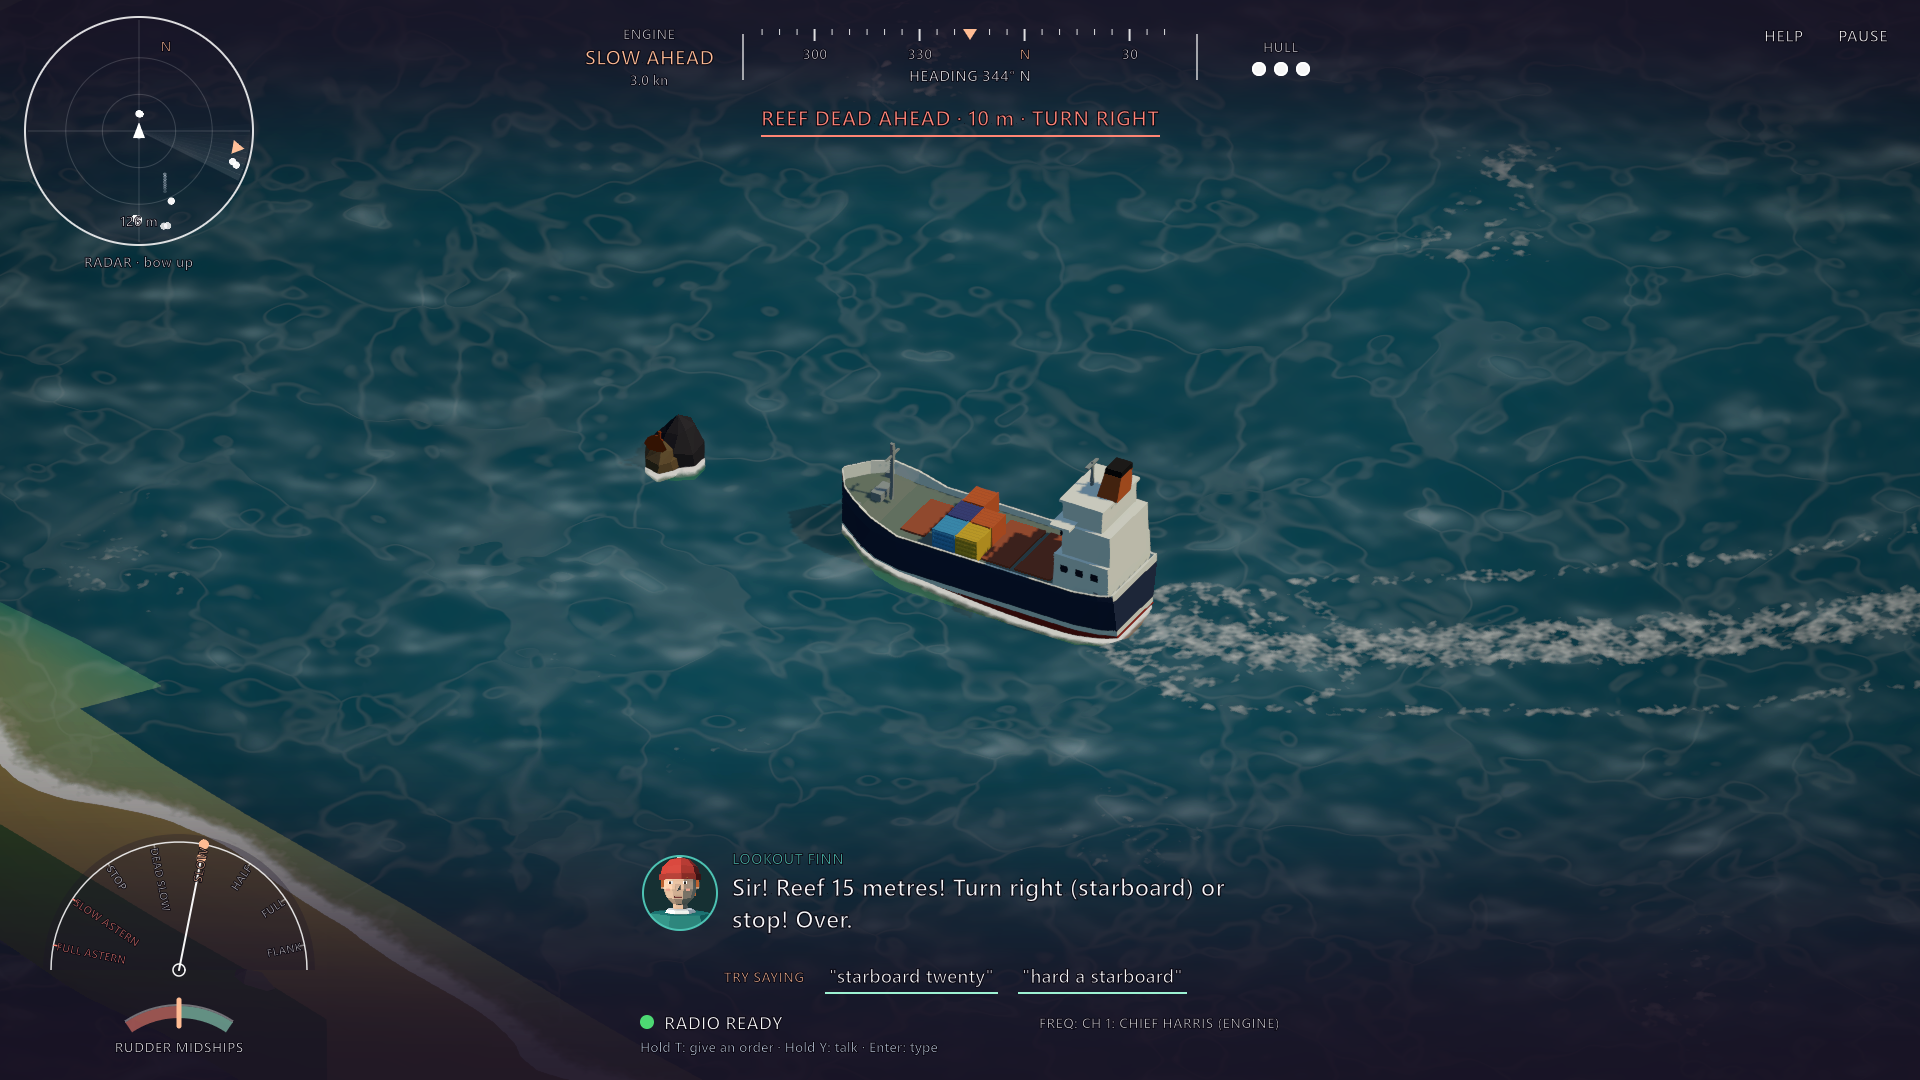
\includegraphics[width=\linewidth]{Document/GameDev/images/Hazard.png}\vspace{0.1cm} &
\textbf{ฉากที่ 4: สถานการณ์เผชิญหน้าสิ่งกีดขวาง}\newline
ระหว่างทางมีอุปสรรค เช่น แนวหินโสโครกหรือทุ่นระเบิดขวางหน้า เรดาร์และยามระวังหน้าส่งสัญญาณเตือนภัยพร้อมบอกระยะและทิศทางที่ควรหลบ ผู้เล่นต้องประเมินสถานการณ์และสั่งการให้ทันเวลา และในโหมดเนื้อเรื่อง ผู้เล่นต้องพูดคำสั่งฉุกเฉินที่แสดงบนจอภายในเวลาที่กำหนด \\ \hline

\vspace{0.1cm}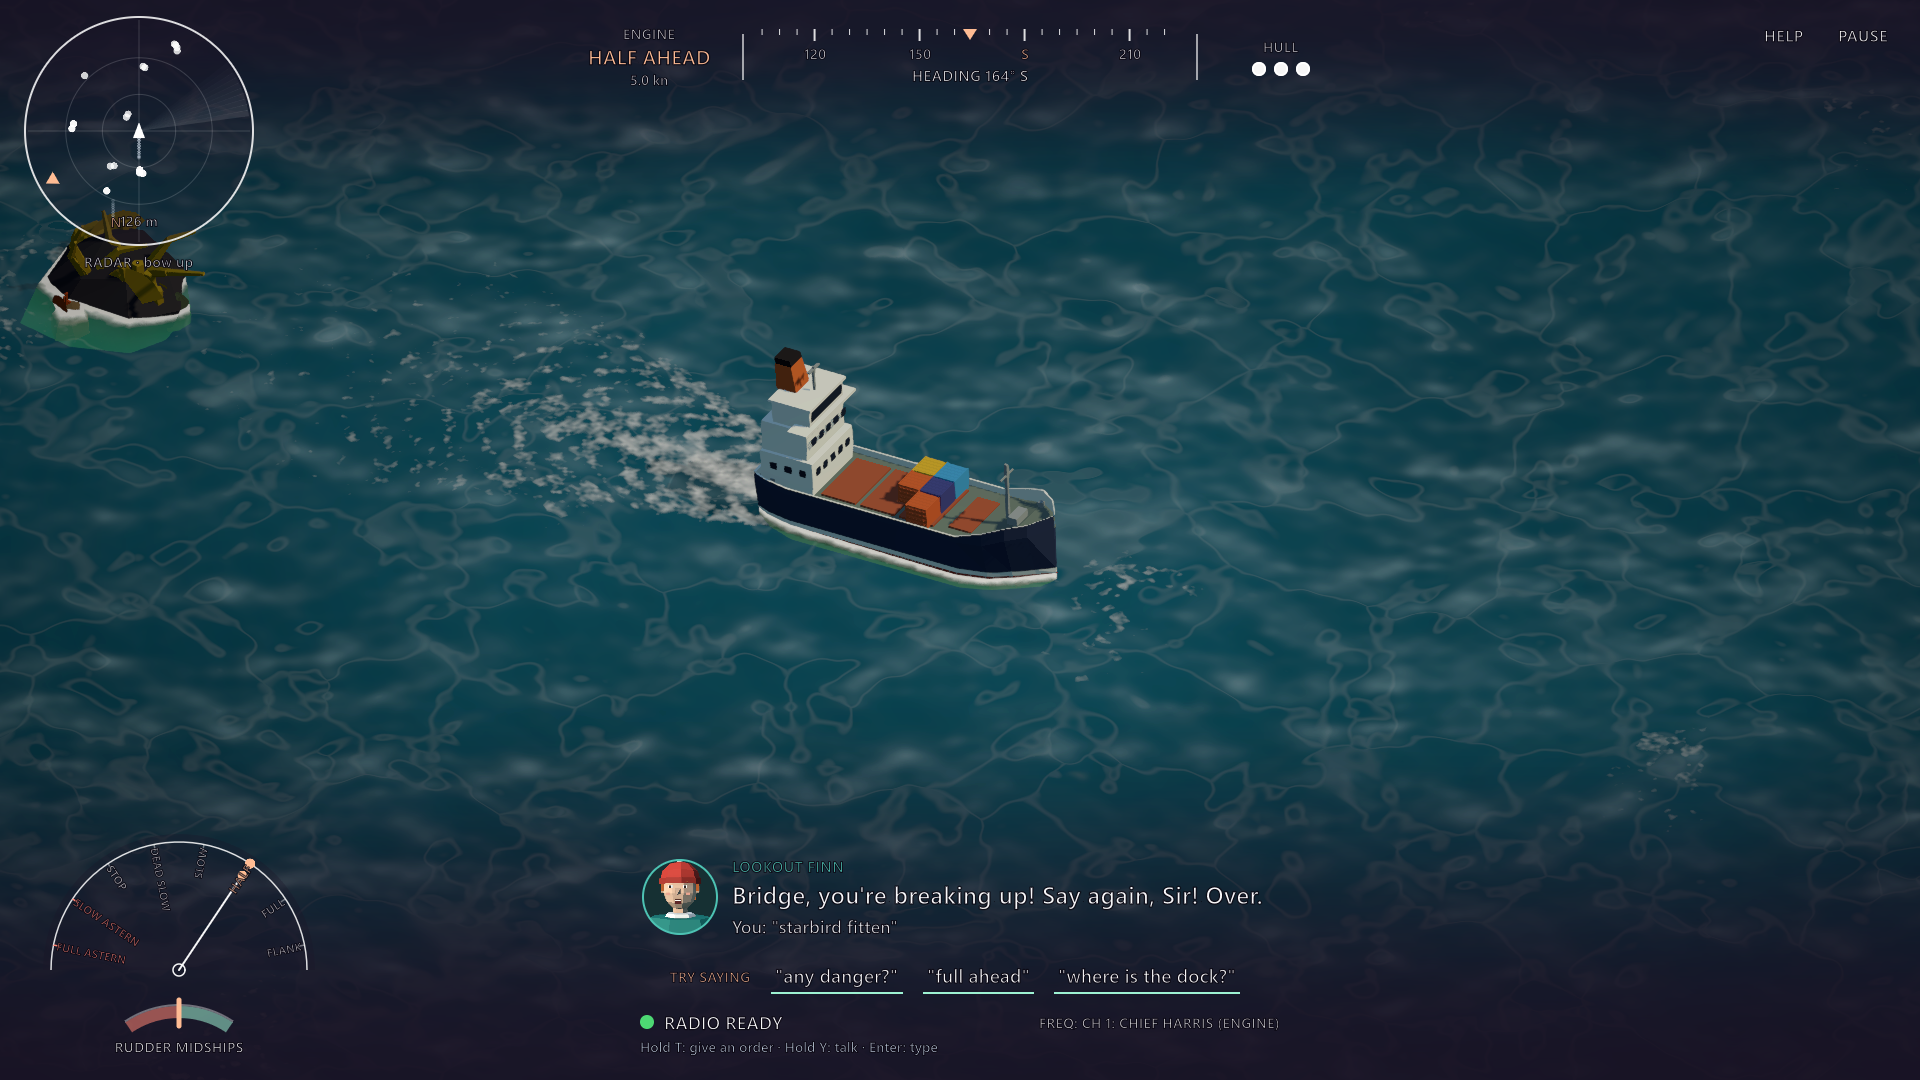
\includegraphics[width=\linewidth]{Document/GameDev/images/Sayagain.png}\vspace{0.1cm} &
\textbf{ฉากที่ 5: สถานการณ์สื่อสารติดขัด (Clarification Request)}\newline
หากผู้เล่นออกเสียงไม่ชัดเจนหรือใช้คำสั่งที่ระบบไม่เข้าใจ ลูกเรือจะขอให้พูดซ้ำ (Say again) เช่น \textit{``Say again, Bridge. Over.''} และให้คำใบ้รูปประโยคมาตรฐานเมื่อไม่เข้าใจติดกัน 2 ครั้ง เพื่อกระตุ้นให้ผู้เล่นแก้ไขการสื่อสารและเปล่งเสียงให้ชัดเจนขึ้น \\ \hline

\vspace{0.1cm}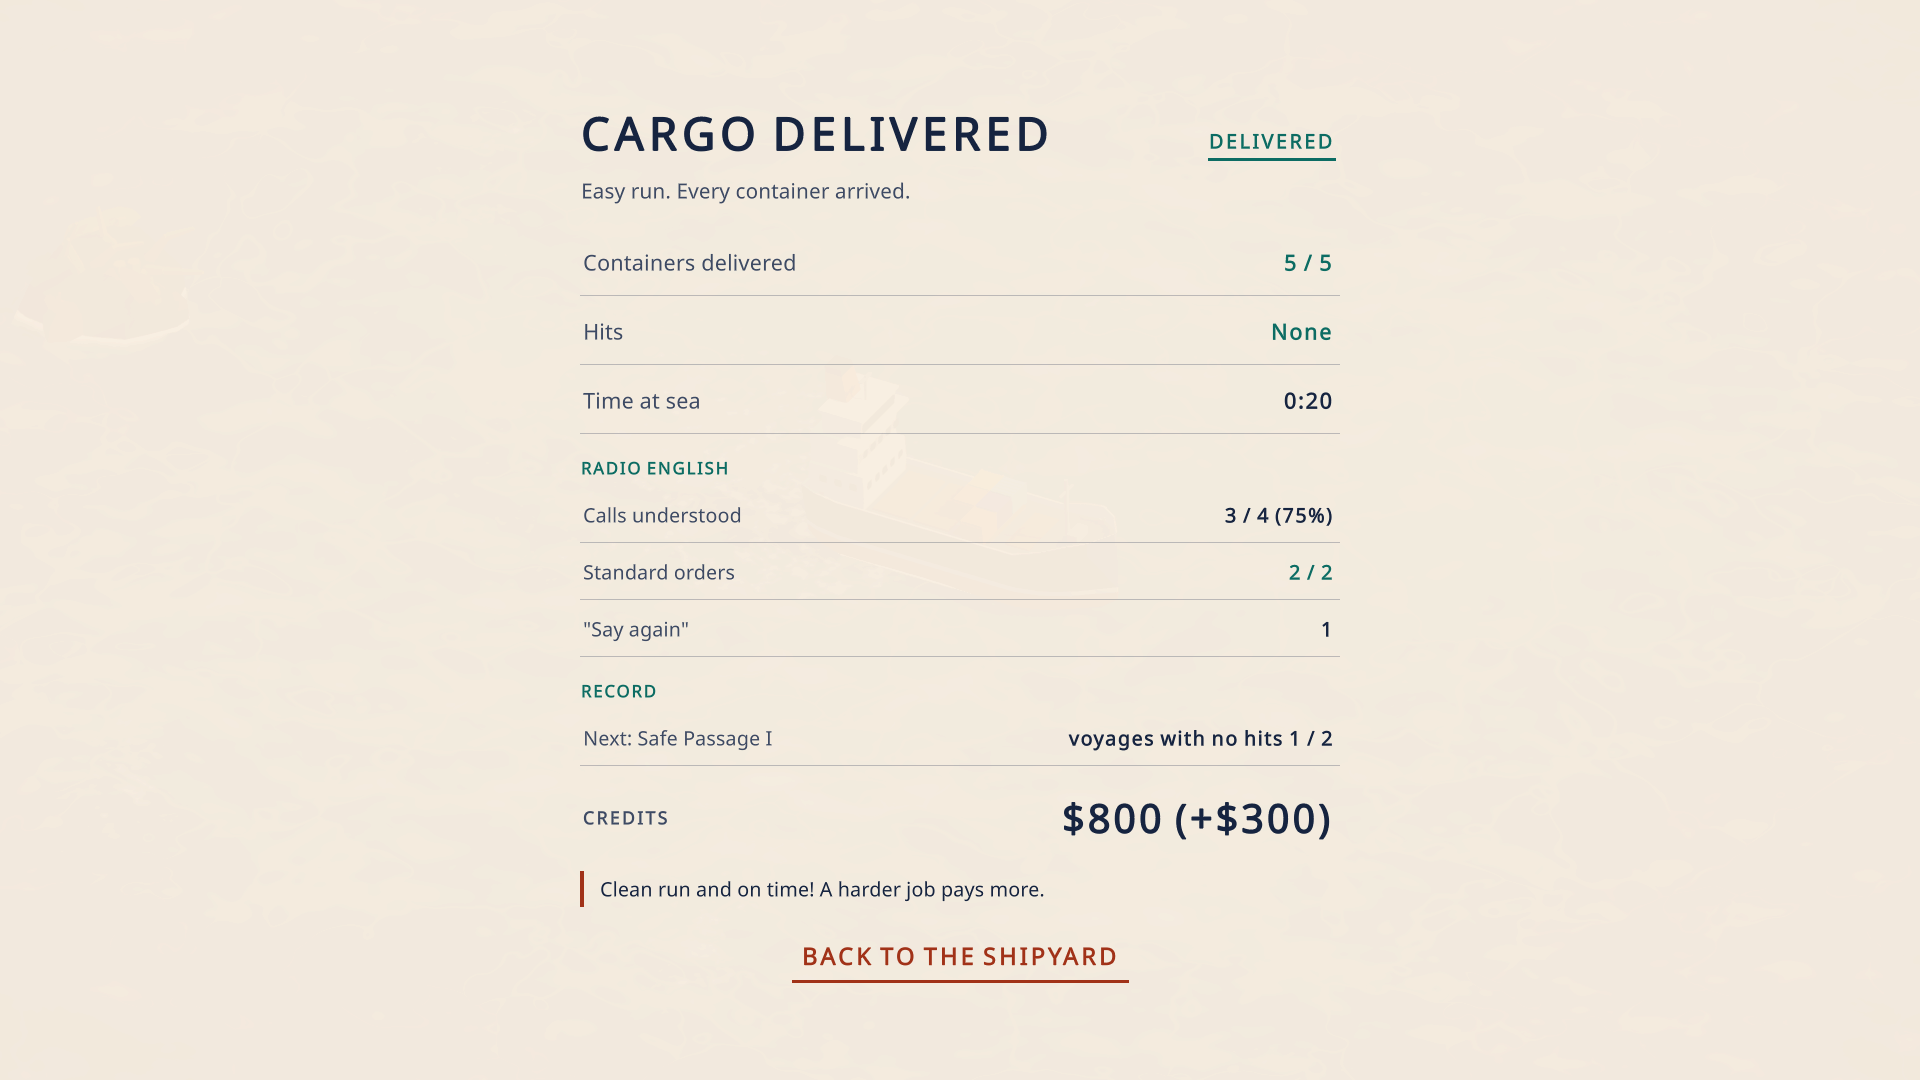
\includegraphics[width=\linewidth]{Document/GameDev/images/Victory.png}\vspace{0.1cm} &
\textbf{ฉากที่ 6: สรุปผลภารกิจ (Result Screen)}\newline
หากนำเรือเทียบท่าและผูกเรือได้สำเร็จ เกมจะแสดงหน้าจอสรุปผล (Cargo Delivered) พร้อมสรุปการสื่อสารภาษาอังกฤษทางวิทยุ ได้แก่ สัดส่วนคำสั่งที่ลูกเรือเข้าใจ จำนวนคำสั่งมาตรฐาน และจำนวนครั้งที่ลูกเรือขอให้พูดซ้ำ แต่หากชนสิ่งกีดขวางจนความทนทานของตัวเรือ (Hull) ลดลงเหลือศูนย์ จะแสดงหน้าจอเรืออับปาง (Ship Lost) และเรือลากจูงจะลากเรือกลับท่าโดยผู้เล่นเสียค่าลากเรือ \\
\hline
\end{tabular}
\end{table}
